\documentclass[a4paper]{book}
\usepackage{makeidx}
\usepackage{natbib}
\usepackage{graphicx}
\usepackage{multicol}
\usepackage{float}
\usepackage{listings}
\usepackage{color}
\usepackage{ifthen}
\usepackage[table]{xcolor}
\usepackage{textcomp}
\usepackage{alltt}
\usepackage{ifpdf}
\ifpdf
\usepackage[pdftex,
            pagebackref=true,
            colorlinks=true,
            linkcolor=blue,
            unicode
           ]{hyperref}
\else
\usepackage[ps2pdf,
            pagebackref=true,
            colorlinks=true,
            linkcolor=blue,
            unicode
           ]{hyperref}
\usepackage{pspicture}
\fi
\usepackage[utf8]{inputenc}
\usepackage{mathptmx}
\usepackage[scaled=.90]{helvet}
\usepackage{courier}
\usepackage{sectsty}
\usepackage[titles]{tocloft}
\usepackage{doxygen}
\lstset{language=C++,inputencoding=utf8,basicstyle=\footnotesize,breaklines=true,breakatwhitespace=true,tabsize=4,numbers=left }
\makeindex
\setcounter{tocdepth}{3}
\renewcommand{\footrulewidth}{0.4pt}
\renewcommand{\familydefault}{\sfdefault}
\hfuzz=15pt
\setlength{\emergencystretch}{15pt}
\hbadness=750
\tolerance=750
\begin{document}
\hypersetup{pageanchor=false,citecolor=blue}
\begin{titlepage}
\vspace*{7cm}
\begin{center}
{\Large 5103 \-Project 1 }\\
\vspace*{1cm}
{\large \-Generated by Doxygen 1.7.6.1}\\
\vspace*{0.5cm}
{\small Mon Feb 13 2012 15:25:25}\\
\end{center}
\end{titlepage}
\clearemptydoublepage
\pagenumbering{roman}
\tableofcontents
\clearemptydoublepage
\pagenumbering{arabic}
\hypersetup{pageanchor=true,citecolor=blue}
\chapter{\-Class \-Index}
\section{\-Class \-Hierarchy}
\-This inheritance list is sorted roughly, but not completely, alphabetically\-:\begin{DoxyCompactList}
\item \contentsline{section}{\-Abstract\-Device}{\pageref{db/d0e/classAbstractDevice}}{}
\begin{DoxyCompactList}
\item \contentsline{section}{\-Block\-Device}{\pageref{db/d6d/classBlockDevice}}{}
\item \contentsline{section}{\-Char\-Device}{\pageref{d8/d4f/classCharDevice}}{}
\item \contentsline{section}{\-Clock\-Device}{\pageref{dc/d14/classClockDevice}}{}
\end{DoxyCompactList}
\item \contentsline{section}{c\-C\-P\-U}{\pageref{d2/dc6/classcCPU}}{}
\item \contentsline{section}{c\-I\-D\-Manager}{\pageref{de/dd4/classcIDManager}}{}
\item \contentsline{section}{c\-Kernel}{\pageref{db/da5/classcKernel}}{}
\item \contentsline{section}{c\-Round\-Robin}{\pageref{dc/dcc/classcRoundRobin}}{}
\item \contentsline{section}{c\-Scheduler}{\pageref{d0/d21/classcScheduler}}{}
\begin{DoxyCompactList}
\item \contentsline{section}{c\-F\-C\-F\-S}{\pageref{d6/dc3/classcFCFS}}{}
\end{DoxyCompactList}
\item \contentsline{section}{fcfs\-Info}{\pageref{d5/d4c/structfcfsInfo}}{}
\item \contentsline{section}{kernel\-Error}{\pageref{dc/d4b/structkernelError}}{}
\item \contentsline{section}{\-Process\-Info}{\pageref{dd/dc8/structProcessInfo}}{}
\end{DoxyCompactList}

\chapter{\-Class \-Index}
\section{\-Class \-List}
\-Here are the classes, structs, unions and interfaces with brief descriptions\-:\begin{DoxyCompactList}
\item\contentsline{section}{\hyperlink{classAbstractDevice}{\-Abstract\-Device} }{\pageref{db/d0e/classAbstractDevice}}{}
\item\contentsline{section}{\hyperlink{classBlockDevice}{\-Block\-Device} }{\pageref{db/d6d/classBlockDevice}}{}
\item\contentsline{section}{\hyperlink{classcCPU}{c\-C\-P\-U} \\*\-A class for emulating a simple cpu }{\pageref{d2/dc6/classcCPU}}{}
\item\contentsline{section}{\hyperlink{classcFCFS}{c\-F\-C\-F\-S} }{\pageref{d6/dc3/classcFCFS}}{}
\item\contentsline{section}{\hyperlink{classCharDevice}{\-Char\-Device} }{\pageref{d8/d4f/classCharDevice}}{}
\item\contentsline{section}{\hyperlink{classcIDManager}{c\-I\-D\-Manager} }{\pageref{de/dd4/classcIDManager}}{}
\item\contentsline{section}{\hyperlink{classcKernel}{c\-Kernel} }{\pageref{db/da5/classcKernel}}{}
\item\contentsline{section}{\hyperlink{classClockDevice}{\-Clock\-Device} }{\pageref{dc/d14/classClockDevice}}{}
\item\contentsline{section}{\hyperlink{classcScheduler}{c\-Scheduler} }{\pageref{d0/d21/classcScheduler}}{}
\item\contentsline{section}{\hyperlink{structProcessInfo}{\-Process\-Info} \\*\-Structure for containing process state and data }{\pageref{dd/dc8/structProcessInfo}}{}
\end{DoxyCompactList}

\chapter{\-File \-Index}
\section{\-File \-List}
\-Here is a list of all documented files with brief descriptions\-:\begin{DoxyCompactList}
\item\contentsline{section}{include/\hyperlink{cpu_8h}{cpu.\-h} }{\pageref{dc/da7/cpu_8h}}{}
\item\contentsline{section}{include/{\bfseries init.\-h} }{\pageref{d8/dc0/init_8h}}{}
\item\contentsline{section}{include/{\bfseries kernel.\-h} }{\pageref{d0/daa/kernel_8h}}{}
\item\contentsline{section}{include/{\bfseries process.\-h} }{\pageref{da/d42/process_8h}}{}
\item\contentsline{section}{include/devices/{\bfseries abstract\-\_\-device.\-h} }{\pageref{d0/d8f/abstract__device_8h}}{}
\item\contentsline{section}{include/devices/{\bfseries block\-\_\-device.\-h} }{\pageref{db/d9a/block__device_8h}}{}
\item\contentsline{section}{include/devices/{\bfseries char\-\_\-device.\-h} }{\pageref{d7/d59/char__device_8h}}{}
\item\contentsline{section}{include/devices/{\bfseries clock\-\_\-device.\-h} }{\pageref{df/d8f/clock__device_8h}}{}
\item\contentsline{section}{include/scheduler/{\bfseries fcfs.\-h} }{\pageref{db/d41/fcfs_8h}}{}
\item\contentsline{section}{include/scheduler/{\bfseries scheduler.\-h} }{\pageref{d2/dd8/scheduler_8h}}{}
\item\contentsline{section}{include/utility/{\bfseries id.\-h} }{\pageref{df/db9/id_8h}}{}
\end{DoxyCompactList}

\chapter{\-Class \-Documentation}
\hypertarget{classAbstractDevice}{\section{\-Abstract\-Device \-Class \-Reference}
\label{db/d0e/classAbstractDevice}\index{\-Abstract\-Device@{\-Abstract\-Device}}
}


\-Inheritance diagram for \-Abstract\-Device\-:\nopagebreak
\begin{figure}[H]
\begin{center}
\leavevmode
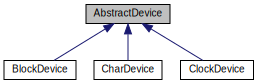
\includegraphics[width=329pt]{dd/d4d/classAbstractDevice__inherit__graph}
\end{center}
\end{figure}
\subsection*{\-Public \-Member \-Functions}
\begin{DoxyCompactItemize}
\item 
\hypertarget{classAbstractDevice_a393c627235e10b16507161febe32cae0}{virtual void {\bfseries set\-Timer} (int time)=0}\label{db/d0e/classAbstractDevice_a393c627235e10b16507161febe32cae0}

\item 
\hypertarget{classAbstractDevice_a4dcc0ef16c540b36a5b628db8f7fe315}{virtual void {\bfseries disarm} ()=0}\label{db/d0e/classAbstractDevice_a4dcc0ef16c540b36a5b628db8f7fe315}

\end{DoxyCompactItemize}


\-The documentation for this class was generated from the following file\-:\begin{DoxyCompactItemize}
\item 
include/devices/abstract\-\_\-device.\-h\end{DoxyCompactItemize}

\hypertarget{classBlockDevice}{\section{\-Block\-Device \-Class \-Reference}
\label{db/d6d/classBlockDevice}\index{\-Block\-Device@{\-Block\-Device}}
}
\-Inheritance diagram for \-Block\-Device\-:\begin{figure}[H]
\begin{center}
\leavevmode
\includegraphics[height=2.000000cm]{db/d6d/classBlockDevice}
\end{center}
\end{figure}
\subsection*{\-Public \-Member \-Functions}
\begin{DoxyCompactItemize}
\item 
\hypertarget{classBlockDevice_a7ff2350ac492e4a73a4b59f9a6bbe629}{void {\bfseries set\-Timer} (int usec)}\label{db/d6d/classBlockDevice_a7ff2350ac492e4a73a4b59f9a6bbe629}

\end{DoxyCompactItemize}


\-The documentation for this class was generated from the following files\-:\begin{DoxyCompactItemize}
\item 
include/devices/block\-\_\-device.\-h\item 
src/devices/block\-\_\-device.\-cpp\end{DoxyCompactItemize}

\hypertarget{classcCPU}{\section{c\-C\-P\-U \-Class \-Reference}
\label{d2/dc6/classcCPU}\index{c\-C\-P\-U@{c\-C\-P\-U}}
}


{\ttfamily \#include $<$cpu.\-h$>$}

\subsection*{\-Public \-Member \-Functions}
\begin{DoxyCompactItemize}
\item 
void \hyperlink{classcCPU_acd957640be8abb7c0d8a24010ed0e737}{set\-Text} (char $\ast$text)
\item 
unsigned int \hyperlink{classcCPU_ab04938ac939d530e521181db6a52944f}{get\-Set\-P\-C} (unsigned int new\-P\-C)
\item 
int \hyperlink{classcCPU_a2d593a0d3d66e532826db4754d5fc4d2}{get\-Set\-V\-C} (int new\-V\-C)
\item 
uint16\-\_\-t \hyperlink{classcCPU_ad485374a709476e2dfb847046d3d5215}{get\-P\-S\-W} ()
\item 
char $\ast$ \hyperlink{classcCPU_a891d9b77e1818ca247e9d76f4db99415}{get\-Param} (int num)
\item 
char \hyperlink{classcCPU_a987e1ab511c71dcde48411f5bb16f9d8}{get\-Opcode} ()
\item 
void \hyperlink{classcCPU_aee300d68026ba9f13d5434ff82f0372a}{run} ()
\end{DoxyCompactItemize}


\subsection{\-Detailed \-Description}
\-A class for emulating a simple cpu.

\-This class emulates the internals of a very simple cpu with two main registers, \-P\-C and \-V\-C. \-In addition, it has other state for handling system calls and program exceptions. 

\subsection{\-Member \-Function \-Documentation}
\hypertarget{classcCPU_a987e1ab511c71dcde48411f5bb16f9d8}{\index{c\-C\-P\-U@{c\-C\-P\-U}!get\-Opcode@{get\-Opcode}}
\index{get\-Opcode@{get\-Opcode}!cCPU@{c\-C\-P\-U}}
\subsubsection[{get\-Opcode}]{\setlength{\rightskip}{0pt plus 5cm}char {\bf c\-C\-P\-U\-::get\-Opcode} (
\begin{DoxyParamCaption}
{}
\end{DoxyParamCaption}
)}}\label{d2/dc6/classcCPU_a987e1ab511c71dcde48411f5bb16f9d8}
\-Get the current \-Opcode

\-Get the current \-Opcode in the cpu. \-This is used by the kernel to determine which system call as being made. \-Used in conjunciton with \hyperlink{classcCPU_a891d9b77e1818ca247e9d76f4db99415}{c\-C\-P\-U\-::get\-Param} the kernel can process system calls. \hypertarget{classcCPU_a891d9b77e1818ca247e9d76f4db99415}{\index{c\-C\-P\-U@{c\-C\-P\-U}!get\-Param@{get\-Param}}
\index{get\-Param@{get\-Param}!cCPU@{c\-C\-P\-U}}
\subsubsection[{get\-Param}]{\setlength{\rightskip}{0pt plus 5cm}char $\ast$ {\bf c\-C\-P\-U\-::get\-Param} (
\begin{DoxyParamCaption}
\item[{int}]{num}
\end{DoxyParamCaption}
)}}\label{d2/dc6/classcCPU_a891d9b77e1818ca247e9d76f4db99415}
\-Get execution parameters from the cpu

\-Fetch the given execution paramter from the cpu's internal buffer. \-When an instruction is encountered that has parameters associated with it, the cpu tokenizes them and places it in an internal buffer. \-This function is mainly used by the kernel in handling system calls.


\begin{DoxyParams}{\-Parameters}
{\em num} & \-Must be less than \-M\-A\-X\-\_\-\-P\-A\-R\-A\-M\-S (currently 2)\\
\hline
\end{DoxyParams}
\begin{DoxyReturn}{\-Returns}
\-Returns a char$\ast$ which points to a string of at most \-M\-A\-X\-\_\-\-P\-A\-R\-A\-M\-\_\-\-S\-I\-Z\-E -\/ 1 bytes. 
\end{DoxyReturn}
\hypertarget{classcCPU_ad485374a709476e2dfb847046d3d5215}{\index{c\-C\-P\-U@{c\-C\-P\-U}!get\-P\-S\-W@{get\-P\-S\-W}}
\index{get\-P\-S\-W@{get\-P\-S\-W}!cCPU@{c\-C\-P\-U}}
\subsubsection[{get\-P\-S\-W}]{\setlength{\rightskip}{0pt plus 5cm}uint16\-\_\-t {\bf c\-C\-P\-U\-::get\-P\-S\-W} (
\begin{DoxyParamCaption}
{}
\end{DoxyParamCaption}
)}}\label{d2/dc6/classcCPU_ad485374a709476e2dfb847046d3d5215}
\-Get the \-Program \-Status \-Word

\-Returns the program status word which is a unsigned 16-\/bit integer type with flags from \hyperlink{cpu_8h_ade10811b11f1c647313bf0a60797a9f9}{e\-P\-S\-W} set. \-These are used by the kernel to make action decisions. \hypertarget{classcCPU_ab04938ac939d530e521181db6a52944f}{\index{c\-C\-P\-U@{c\-C\-P\-U}!get\-Set\-P\-C@{get\-Set\-P\-C}}
\index{get\-Set\-P\-C@{get\-Set\-P\-C}!cCPU@{c\-C\-P\-U}}
\subsubsection[{get\-Set\-P\-C}]{\setlength{\rightskip}{0pt plus 5cm}unsigned int {\bf c\-C\-P\-U\-::get\-Set\-P\-C} (
\begin{DoxyParamCaption}
\item[{unsigned int}]{new\-P\-C}
\end{DoxyParamCaption}
)}}\label{d2/dc6/classcCPU_ab04938ac939d530e521181db6a52944f}
\-Get/\-Set the program counter

\-Get the current value for the program counter and then set its value to the given parameter. \-This is useful for swapping out process values. \hypertarget{classcCPU_a2d593a0d3d66e532826db4754d5fc4d2}{\index{c\-C\-P\-U@{c\-C\-P\-U}!get\-Set\-V\-C@{get\-Set\-V\-C}}
\index{get\-Set\-V\-C@{get\-Set\-V\-C}!cCPU@{c\-C\-P\-U}}
\subsubsection[{get\-Set\-V\-C}]{\setlength{\rightskip}{0pt plus 5cm}int {\bf c\-C\-P\-U\-::get\-Set\-V\-C} (
\begin{DoxyParamCaption}
\item[{int}]{new\-V\-C}
\end{DoxyParamCaption}
)}}\label{d2/dc6/classcCPU_a2d593a0d3d66e532826db4754d5fc4d2}
\-Get/\-Set the \-V\-C

\-Get the current value for \-V\-C and set its value to the given paramter. \-This is useful for swapping out process values. \hypertarget{classcCPU_aee300d68026ba9f13d5434ff82f0372a}{\index{c\-C\-P\-U@{c\-C\-P\-U}!run@{run}}
\index{run@{run}!cCPU@{c\-C\-P\-U}}
\subsubsection[{run}]{\setlength{\rightskip}{0pt plus 5cm}void {\bf c\-C\-P\-U\-::run} (
\begin{DoxyParamCaption}
{}
\end{DoxyParamCaption}
)}}\label{d2/dc6/classcCPU_aee300d68026ba9f13d5434ff82f0372a}
\-Start execution

\-Once all appropriate process data is entered by the kernel this function is called to start execution. \-Any time control needs to be returned to the kernel this function will return with the appropriate \-P\-S\-W flags set for the kernel to act on. \hypertarget{classcCPU_acd957640be8abb7c0d8a24010ed0e737}{\index{c\-C\-P\-U@{c\-C\-P\-U}!set\-Text@{set\-Text}}
\index{set\-Text@{set\-Text}!cCPU@{c\-C\-P\-U}}
\subsubsection[{set\-Text}]{\setlength{\rightskip}{0pt plus 5cm}void {\bf c\-C\-P\-U\-::set\-Text} (
\begin{DoxyParamCaption}
\item[{char $\ast$}]{text}
\end{DoxyParamCaption}
)}}\label{d2/dc6/classcCPU_acd957640be8abb7c0d8a24010ed0e737}
\-Set the program text

\-Point the cpu to the text data for the running process. \-This text is indexed using the program counter (\-P\-C).


\begin{DoxyParams}{\-Parameters}
{\em text} & \-Program text pointer. assert( text != \-N\-U\-L\-L) \\
\hline
\end{DoxyParams}


\-The documentation for this class was generated from the following files\-:\begin{DoxyCompactItemize}
\item 
include/\hyperlink{cpu_8h}{cpu.\-h}\item 
src/cpu.\-cpp\end{DoxyCompactItemize}

\hypertarget{classcFCFS}{\section{c\-F\-C\-F\-S \-Class \-Reference}
\label{d6/dc3/classcFCFS}\index{c\-F\-C\-F\-S@{c\-F\-C\-F\-S}}
}


\-Inheritance diagram for c\-F\-C\-F\-S\-:\nopagebreak
\begin{figure}[H]
\begin{center}
\leavevmode
\includegraphics[width=144pt]{d2/d94/classcFCFS__inherit__graph}
\end{center}
\end{figure}


\-Collaboration diagram for c\-F\-C\-F\-S\-:\nopagebreak
\begin{figure}[H]
\begin{center}
\leavevmode
\includegraphics[width=303pt]{d4/d8d/classcFCFS__coll__graph}
\end{center}
\end{figure}
\subsection*{\-Public \-Member \-Functions}
\begin{DoxyCompactItemize}
\item 
\hypertarget{classcFCFS_aff34f18c6f4c3f38029d904cd2ec55de}{void {\bfseries init\-Proc\-Schedule\-Info} (\hyperlink{structProcessInfo}{\-Process\-Info} $\ast$)}\label{d6/dc3/classcFCFS_aff34f18c6f4c3f38029d904cd2ec55de}

\item 
\hypertarget{classcFCFS_a25d4bf440041f5294f3b9c5aff20b411}{void {\bfseries add\-Process} (\hyperlink{structProcessInfo}{\-Process\-Info} $\ast$)}\label{d6/dc3/classcFCFS_a25d4bf440041f5294f3b9c5aff20b411}

\item 
\hypertarget{classcFCFS_a1b8ee3a759a31032ec7c1cd7b15ed5df}{void {\bfseries set\-Blocked} (\hyperlink{structProcessInfo}{\-Process\-Info} $\ast$)}\label{d6/dc3/classcFCFS_a1b8ee3a759a31032ec7c1cd7b15ed5df}

\item 
\hypertarget{classcFCFS_a793da0298f9b36ab8505a0e3daaf41ec}{void {\bfseries unblock\-Process} (\hyperlink{structProcessInfo}{\-Process\-Info} $\ast$)}\label{d6/dc3/classcFCFS_a793da0298f9b36ab8505a0e3daaf41ec}

\item 
\hypertarget{classcFCFS_aeeac757885108ae510b728600ebba248}{void {\bfseries remove\-Process} (\hyperlink{structProcessInfo}{\-Process\-Info} $\ast$)}\label{d6/dc3/classcFCFS_aeeac757885108ae510b728600ebba248}

\item 
\hypertarget{classcFCFS_aa2b92a8a992078e499aab455c9d78faf}{\hyperlink{structProcessInfo}{\-Process\-Info} $\ast$ {\bfseries get\-Next\-To\-Run} ()}\label{d6/dc3/classcFCFS_aa2b92a8a992078e499aab455c9d78faf}

\item 
\hypertarget{classcFCFS_a0a72de791436a84120a534dd2fa0485d}{pid\-Type {\bfseries num\-Processes} ()}\label{d6/dc3/classcFCFS_a0a72de791436a84120a534dd2fa0485d}

\end{DoxyCompactItemize}
\subsection*{\-Private \-Attributes}
\begin{DoxyCompactItemize}
\item 
\hypertarget{classcFCFS_afebe08e2ae6dc564b5aad24e3b30f842}{queue$<$ \hyperlink{structProcessInfo}{\-Process\-Info} $\ast$ $>$ {\bfseries ready\-Queue}}\label{d6/dc3/classcFCFS_afebe08e2ae6dc564b5aad24e3b30f842}

\item 
\hypertarget{classcFCFS_af61586b3ed208ebd0e12bc495c31b56c}{queue$<$ \hyperlink{structProcessInfo}{\-Process\-Info} $\ast$ $>$ {\bfseries blocked\-Queue}}\label{d6/dc3/classcFCFS_af61586b3ed208ebd0e12bc495c31b56c}

\end{DoxyCompactItemize}


\-The documentation for this class was generated from the following files\-:\begin{DoxyCompactItemize}
\item 
include/scheduler/fcfs.\-h\item 
src/scheduler/fcfs.\-cpp\end{DoxyCompactItemize}

\hypertarget{classCharDevice}{\section{\-Char\-Device \-Class \-Reference}
\label{d8/d4f/classCharDevice}\index{\-Char\-Device@{\-Char\-Device}}
}


\-Inheritance diagram for \-Char\-Device\-:\nopagebreak
\begin{figure}[H]
\begin{center}
\leavevmode
\includegraphics[width=162pt]{da/d98/classCharDevice__inherit__graph}
\end{center}
\end{figure}


\-Collaboration diagram for \-Char\-Device\-:\nopagebreak
\begin{figure}[H]
\begin{center}
\leavevmode
\includegraphics[width=162pt]{d2/db9/classCharDevice__coll__graph}
\end{center}
\end{figure}
\subsection*{\-Public \-Member \-Functions}
\begin{DoxyCompactItemize}
\item 
\hypertarget{classCharDevice_a8689c0a03b971367322a9dd25bcfb7db}{void {\bfseries set\-Timer} (int usec)}\label{d8/d4f/classCharDevice_a8689c0a03b971367322a9dd25bcfb7db}

\end{DoxyCompactItemize}


\-The documentation for this class was generated from the following files\-:\begin{DoxyCompactItemize}
\item 
include/devices/char\-\_\-device.\-h\item 
src/devices/char\-\_\-device.\-cpp\end{DoxyCompactItemize}

\hypertarget{classcIDManager}{\section{c\-I\-D\-Manager \-Class \-Reference}
\label{de/dd4/classcIDManager}\index{c\-I\-D\-Manager@{c\-I\-D\-Manager}}
}
\subsection*{\-Public \-Member \-Functions}
\begin{DoxyCompactItemize}
\item 
\hyperlink{classcIDManager_a59021595aaf85ebc151c207a8a04f101}{c\-I\-D\-Manager} (unsigned int start\-I\-D=0)
\item 
unsigned int \hyperlink{classcIDManager_a45420147e785cc219743e9aa2c336501}{get\-I\-D} ()
\item 
void \hyperlink{classcIDManager_a6671d898740f88cf40860b0b9e119b02}{return\-I\-D} (unsigned int id)
\end{DoxyCompactItemize}


\subsection{\-Constructor \& \-Destructor \-Documentation}
\hypertarget{classcIDManager_a59021595aaf85ebc151c207a8a04f101}{\index{c\-I\-D\-Manager@{c\-I\-D\-Manager}!c\-I\-D\-Manager@{c\-I\-D\-Manager}}
\index{c\-I\-D\-Manager@{c\-I\-D\-Manager}!cIDManager@{c\-I\-D\-Manager}}
\subsubsection[{c\-I\-D\-Manager}]{\setlength{\rightskip}{0pt plus 5cm}{\bf c\-I\-D\-Manager\-::c\-I\-D\-Manager} (
\begin{DoxyParamCaption}
\item[{unsigned int}]{start\-I\-D = {\ttfamily 0}}
\end{DoxyParamCaption}
)}}\label{de/dd4/classcIDManager_a59021595aaf85ebc151c207a8a04f101}
\-Creates a new \-I\-D \-Manager object

\-Default start \-I\-D is 0. 

\subsection{\-Member \-Function \-Documentation}
\hypertarget{classcIDManager_a45420147e785cc219743e9aa2c336501}{\index{c\-I\-D\-Manager@{c\-I\-D\-Manager}!get\-I\-D@{get\-I\-D}}
\index{get\-I\-D@{get\-I\-D}!cIDManager@{c\-I\-D\-Manager}}
\subsubsection[{get\-I\-D}]{\setlength{\rightskip}{0pt plus 5cm}unsigned int {\bf c\-I\-D\-Manager\-::get\-I\-D} (
\begin{DoxyParamCaption}
{}
\end{DoxyParamCaption}
)}}\label{de/dd4/classcIDManager_a45420147e785cc219743e9aa2c336501}
\-Reserves a unique \-I\-D

\-Unique is in the sense that no one else is currently using it but it may have been used previously. are distributed in increasing order until \-U\-I\-N\-T\-\_\-\-M\-A\-X is reached. \-After this is reached, \-I\-Ds are given from the queue of returned \-I\-Ds. \-If this queue is empty then an exception is thrown. \hypertarget{classcIDManager_a6671d898740f88cf40860b0b9e119b02}{\index{c\-I\-D\-Manager@{c\-I\-D\-Manager}!return\-I\-D@{return\-I\-D}}
\index{return\-I\-D@{return\-I\-D}!cIDManager@{c\-I\-D\-Manager}}
\subsubsection[{return\-I\-D}]{\setlength{\rightskip}{0pt plus 5cm}void {\bf c\-I\-D\-Manager\-::return\-I\-D} (
\begin{DoxyParamCaption}
\item[{unsigned int}]{id}
\end{DoxyParamCaption}
)}}\label{de/dd4/classcIDManager_a6671d898740f88cf40860b0b9e119b02}
\-Returns an \-I\-D to the manager

\-If the \-I\-D is not equal to the one last given then it is added to a 'free queue'. \-If it is equal to the last one reserved then the \-I\-D counter is simply decremented \-If this last case happens, it causes \hyperlink{classcIDManager_a45420147e785cc219743e9aa2c336501}{c\-I\-D\-Manager\-::get\-I\-D} to stop consuming from the queue and return this newly availabe \-I\-D. 

\-The documentation for this class was generated from the following files\-:\begin{DoxyCompactItemize}
\item 
include/utility/id.\-h\item 
src/utility/id.\-cpp\end{DoxyCompactItemize}

\hypertarget{classcKernel}{\section{c\-Kernel \-Class \-Reference}
\label{db/da5/classcKernel}\index{c\-Kernel@{c\-Kernel}}
}


\-Collaboration diagram for c\-Kernel\-:\nopagebreak
\begin{figure}[H]
\begin{center}
\leavevmode
\includegraphics[width=350pt]{d4/d6f/classcKernel__coll__graph}
\end{center}
\end{figure}
\subsection*{\-Public \-Member \-Functions}
\begin{DoxyCompactItemize}
\item 
\hyperlink{classcKernel_a64d105a595a4d14a47bb65426b331159}{c\-Kernel} ()
\begin{DoxyCompactList}\small\item\em \-Default \hyperlink{classcKernel}{c\-Kernel} constructor. \end{DoxyCompactList}\item 
void \hyperlink{classcKernel_a0ce9a2721bb1ea4d7f999198634f702d}{boot} ()
\begin{DoxyCompactList}\small\item\em \-Start the '\-O\-S' \-Kernel. \end{DoxyCompactList}\item 
void \hyperlink{classcKernel_a5440eace2647ffd5279de55600947b84}{init\-Process} (const char $\ast$filename, pid\-Type parent, int priority=\hyperlink{kernel_8h_a0756f011ef667460d583017366823244}{\-D\-E\-F\-A\-U\-L\-T\-\_\-\-P\-R\-I\-O\-R\-I\-T\-Y})
\begin{DoxyCompactList}\small\item\em \-Initialize a \-Process. \end{DoxyCompactList}\item 
void \hyperlink{classcKernel_a1e7cb5c6d9e6140e197f9b18dc8bd1b1}{cleanup\-Process} (pid\-Type pid)
\begin{DoxyCompactList}\small\item\em \-Cleans up a terminated process. \end{DoxyCompactList}\item 
\hypertarget{classcKernel_acdaa8be94f13fcb1f11b3bf90bc316fa}{void {\bfseries \-\_\-sys\-Call} (const char call)}\label{db/da5/classcKernel_acdaa8be94f13fcb1f11b3bf90bc316fa}

\end{DoxyCompactItemize}
\subsection*{\-Private \-Member \-Functions}
\begin{DoxyCompactItemize}
\item 
void \hyperlink{classcKernel_a1b8e06f240c1bb7d0c4d0d30bcc55e18}{swap\-Processes} (\hyperlink{structProcessInfo}{\-Process\-Info} $\ast$proc, bool switch\-Mode=true)
\begin{DoxyCompactList}\small\item\em \-Swap a process on the cpu. \end{DoxyCompactList}\item 
\hypertarget{classcKernel_abcc0464e62a5fb82ddf4a3f8ba5ec461}{void {\bfseries cleanup\-Process} (\hyperlink{structProcessInfo}{\-Process\-Info} $\ast$)}\label{db/da5/classcKernel_abcc0464e62a5fb82ddf4a3f8ba5ec461}

\item 
void \hyperlink{classcKernel_a60ccaffeee3cfcfdfb4aa7b9e33b19f4}{sig\-Handler} (int signum, siginfo\-\_\-t $\ast$info)
\begin{DoxyCompactList}\small\item\em \-Handler for all signals. \end{DoxyCompactList}\end{DoxyCompactItemize}
\subsection*{\-Static \-Private \-Member \-Functions}
\begin{DoxyCompactItemize}
\item 
\hypertarget{classcKernel_a571bb344ba50970d9c4a1cb5b500bbcd}{static void {\bfseries sig\-\_\-catch} (int signum, siginfo\-\_\-t $\ast$info, void $\ast$context)}\label{db/da5/classcKernel_a571bb344ba50970d9c4a1cb5b500bbcd}

\end{DoxyCompactItemize}
\subsection*{\-Private \-Attributes}
\begin{DoxyCompactItemize}
\item 
\hypertarget{classcKernel_a7b4ac330752179e72a5e440d30c64e91}{\-F\-I\-L\-E $\ast$ {\bfseries trace\-Stream}}\label{db/da5/classcKernel_a7b4ac330752179e72a5e440d30c64e91}

\item 
\hypertarget{classcKernel_a1fb233fa1c51650ccf2c872d856329ff}{\hyperlink{classcCPU}{c\-C\-P\-U} {\bfseries cpu}}\label{db/da5/classcKernel_a1fb233fa1c51650ccf2c872d856329ff}

\item 
\hypertarget{classcKernel_a1de4acdb706016573445b3c497e3b508}{int {\bfseries clock\-Tick}}\label{db/da5/classcKernel_a1de4acdb706016573445b3c497e3b508}

\item 
\hypertarget{classcKernel_a6b669b48db537f392164b9fcf3109e87}{pthread\-\_\-barrier\-\_\-t {\bfseries tick\-Barrier}}\label{db/da5/classcKernel_a6b669b48db537f392164b9fcf3109e87}

\item 
\hypertarget{classcKernel_a2d05550b96d1a4c4b02d523574fa94b3}{\hyperlink{classBlockDevice}{\-Block\-Device} {\bfseries b\-Device}}\label{db/da5/classcKernel_a2d05550b96d1a4c4b02d523574fa94b3}

\item 
\hypertarget{classcKernel_abe168524c497a731b708eeeffa810a4b}{\hyperlink{classCharDevice}{\-Char\-Device} {\bfseries c\-Device}}\label{db/da5/classcKernel_abe168524c497a731b708eeeffa810a4b}

\item 
\hypertarget{classcKernel_a1e82363115819c11c74ac261d82d11b5}{\hyperlink{classClockDevice}{\-Clock\-Device} {\bfseries clock\-Interrupt}}\label{db/da5/classcKernel_a1e82363115819c11c74ac261d82d11b5}

\item 
\hypertarget{classcKernel_a6e33ce858b1839bbeb6503515bf11475}{\hyperlink{structProcessInfo}{\-Process\-Info} $\ast$ \hyperlink{classcKernel_a6e33ce858b1839bbeb6503515bf11475}{running\-Proc}}\label{db/da5/classcKernel_a6e33ce858b1839bbeb6503515bf11475}

\begin{DoxyCompactList}\small\item\em \hyperlink{structProcessInfo}{\-Process\-Info} \end{DoxyCompactList}\item 
\hypertarget{classcKernel_a03d2c6943661797e86c030864890183e}{\hyperlink{classcIDManager}{c\-I\-D\-Manager} {\bfseries id\-Generator}}\label{db/da5/classcKernel_a03d2c6943661797e86c030864890183e}

\item 
\hypertarget{classcKernel_a739c2652aee254fc800e8fe05452db8c}{\hyperlink{classcFCFS}{scheduler\-Type} {\bfseries scheduler}}\label{db/da5/classcKernel_a739c2652aee254fc800e8fe05452db8c}

\end{DoxyCompactItemize}
\subsection*{\-Static \-Private \-Attributes}
\begin{DoxyCompactItemize}
\item 
\hypertarget{classcKernel_ae757ff0479ba7ce5154aff58f493cfa9}{static \hyperlink{classcKernel}{c\-Kernel} $\ast$ {\bfseries kernel\-\_\-instance}}\label{db/da5/classcKernel_ae757ff0479ba7ce5154aff58f493cfa9}

\end{DoxyCompactItemize}


\subsection{\-Constructor \& \-Destructor \-Documentation}
\hypertarget{classcKernel_a64d105a595a4d14a47bb65426b331159}{\index{c\-Kernel@{c\-Kernel}!c\-Kernel@{c\-Kernel}}
\index{c\-Kernel@{c\-Kernel}!cKernel@{c\-Kernel}}
\subsubsection[{c\-Kernel}]{\setlength{\rightskip}{0pt plus 5cm}{\bf c\-Kernel\-::c\-Kernel} (
\begin{DoxyParamCaption}
{}
\end{DoxyParamCaption}
)}}\label{db/da5/classcKernel_a64d105a595a4d14a47bb65426b331159}
\-The default constructor initializes all internal datastructures and loads the initial program (default\-: 'main.\-trace') but does not run it. 

\subsection{\-Member \-Function \-Documentation}
\hypertarget{classcKernel_a0ce9a2721bb1ea4d7f999198634f702d}{\index{c\-Kernel@{c\-Kernel}!boot@{boot}}
\index{boot@{boot}!cKernel@{c\-Kernel}}
\subsubsection[{boot}]{\setlength{\rightskip}{0pt plus 5cm}void {\bf c\-Kernel\-::boot} (
\begin{DoxyParamCaption}
{}
\end{DoxyParamCaption}
)}}\label{db/da5/classcKernel_a0ce9a2721bb1ea4d7f999198634f702d}
\-Starts the main kernel loop. \-The initial program is loaded and execution follows from there.


\begin{DoxyExceptions}{\-Exceptions}
{\em \hyperlink{structkernelError}{kernel\-Error}} & \\
\hline
\end{DoxyExceptions}
\hypertarget{classcKernel_a1e7cb5c6d9e6140e197f9b18dc8bd1b1}{\index{c\-Kernel@{c\-Kernel}!cleanup\-Process@{cleanup\-Process}}
\index{cleanup\-Process@{cleanup\-Process}!cKernel@{c\-Kernel}}
\subsubsection[{cleanup\-Process}]{\setlength{\rightskip}{0pt plus 5cm}void c\-Kernel\-::cleanup\-Process (
\begin{DoxyParamCaption}
\item[{pid\-Type}]{pid}
\end{DoxyParamCaption}
)}}\label{db/da5/classcKernel_a1e7cb5c6d9e6140e197f9b18dc8bd1b1}
\-Cleans up any memory and kernel entries associated with the terminated process. \-Also removes the process from the scheduler. \hypertarget{classcKernel_a5440eace2647ffd5279de55600947b84}{\index{c\-Kernel@{c\-Kernel}!init\-Process@{init\-Process}}
\index{init\-Process@{init\-Process}!cKernel@{c\-Kernel}}
\subsubsection[{init\-Process}]{\setlength{\rightskip}{0pt plus 5cm}void {\bf c\-Kernel\-::init\-Process} (
\begin{DoxyParamCaption}
\item[{const char $\ast$}]{filename, }
\item[{pid\-Type}]{parent, }
\item[{int}]{priority = {\ttfamily {\bf \-D\-E\-F\-A\-U\-L\-T\-\_\-\-P\-R\-I\-O\-R\-I\-T\-Y}}}
\end{DoxyParamCaption}
)}}\label{db/da5/classcKernel_a5440eace2647ffd5279de55600947b84}
\-Initializes a process by loading program file contents, setting default process values and adding it in a ready state to the scheduler. \hypertarget{classcKernel_a60ccaffeee3cfcfdfb4aa7b9e33b19f4}{\index{c\-Kernel@{c\-Kernel}!sig\-Handler@{sig\-Handler}}
\index{sig\-Handler@{sig\-Handler}!cKernel@{c\-Kernel}}
\subsubsection[{sig\-Handler}]{\setlength{\rightskip}{0pt plus 5cm}void {\bf c\-Kernel\-::sig\-Handler} (
\begin{DoxyParamCaption}
\item[{int}]{signum, }
\item[{siginfo\-\_\-t $\ast$}]{info}
\end{DoxyParamCaption}
)\hspace{0.3cm}{\ttfamily  \mbox{[}private\mbox{]}}}}\label{db/da5/classcKernel_a60ccaffeee3cfcfdfb4aa7b9e33b19f4}
\-Each device uses a timer from \-S\-I\-G\-R\-T\-M\-I\-N -\/$>$ \-S\-I\-G\-R\-T\-M\-A\-X. \-Because these are not required to be compile time constants, a switch statement cannot be used. \-When a signal is received by the kernel, careful consideration must be made to the current state. \-Below is each signal and how it is handled\-: \hypertarget{classcKernel_a1b8e06f240c1bb7d0c4d0d30bcc55e18}{\index{c\-Kernel@{c\-Kernel}!swap\-Processes@{swap\-Processes}}
\index{swap\-Processes@{swap\-Processes}!cKernel@{c\-Kernel}}
\subsubsection[{swap\-Processes}]{\setlength{\rightskip}{0pt plus 5cm}void {\bf c\-Kernel\-::swap\-Processes} (
\begin{DoxyParamCaption}
\item[{{\bf \-Process\-Info} $\ast$}]{proc, }
\item[{bool}]{switch\-Mode = {\ttfamily true}}
\end{DoxyParamCaption}
)\hspace{0.3cm}{\ttfamily  \mbox{[}private\mbox{]}}}}\label{db/da5/classcKernel_a1b8e06f240c1bb7d0c4d0d30bcc55e18}
\-Takes the process in its parameter and swaps it with the one currently running in the cpu. 

\-The documentation for this class was generated from the following files\-:\begin{DoxyCompactItemize}
\item 
include/\hyperlink{kernel_8h}{kernel.\-h}\item 
src/kernel.\-cpp\end{DoxyCompactItemize}

\hypertarget{classClockDevice}{\section{\-Clock\-Device \-Class \-Reference}
\label{dc/d14/classClockDevice}\index{\-Clock\-Device@{\-Clock\-Device}}
}
\-Inheritance diagram for \-Clock\-Device\-:\begin{figure}[H]
\begin{center}
\leavevmode
\includegraphics[height=2.000000cm]{dc/d14/classClockDevice}
\end{center}
\end{figure}
\subsection*{\-Public \-Member \-Functions}
\begin{DoxyCompactItemize}
\item 
\hypertarget{classClockDevice_a780eebde86fb6a6400894128ac37fa37}{void {\bfseries set\-Timer} (int usec)}\label{dc/d14/classClockDevice_a780eebde86fb6a6400894128ac37fa37}

\end{DoxyCompactItemize}


\-The documentation for this class was generated from the following files\-:\begin{DoxyCompactItemize}
\item 
include/devices/clock\-\_\-device.\-h\item 
src/devices/clock\-\_\-device.\-cpp\end{DoxyCompactItemize}

\hypertarget{classcRoundRobin}{\section{c\-Round\-Robin \-Class \-Reference}
\label{dc/dcc/classcRoundRobin}\index{c\-Round\-Robin@{c\-Round\-Robin}}
}
\subsection*{\-Public \-Member \-Functions}
\begin{DoxyCompactItemize}
\item 
\hypertarget{classcRoundRobin_aadb221df9b12f61c3151996ea5c09741}{void {\bfseries init\-Proc\-Schedule\-Info} (\hyperlink{structProcessInfo}{\-Process\-Info} $\ast$)}\label{dc/dcc/classcRoundRobin_aadb221df9b12f61c3151996ea5c09741}

\item 
\hypertarget{classcRoundRobin_a3571d05a8daebccb758d63b8327f8a22}{void {\bfseries add\-Process} (\hyperlink{structProcessInfo}{\-Process\-Info} $\ast$)}\label{dc/dcc/classcRoundRobin_a3571d05a8daebccb758d63b8327f8a22}

\item 
\hypertarget{classcRoundRobin_a13609de0f36c81a780072f9c0730f963}{void {\bfseries set\-Blocked} (\hyperlink{structProcessInfo}{\-Process\-Info} $\ast$)}\label{dc/dcc/classcRoundRobin_a13609de0f36c81a780072f9c0730f963}

\item 
\hypertarget{classcRoundRobin_a81d0cd6050ebff3c72ca1e829f2d4991}{void {\bfseries unblocked\-Process} (\hyperlink{structProcessInfo}{\-Process\-Info} $\ast$)}\label{dc/dcc/classcRoundRobin_a81d0cd6050ebff3c72ca1e829f2d4991}

\item 
\hypertarget{classcRoundRobin_a1bc7bfc4c36bdbe3f3938810817d885e}{void {\bfseries remove\-Process} (\hyperlink{structProcessInfo}{\-Process\-Info} $\ast$)}\label{dc/dcc/classcRoundRobin_a1bc7bfc4c36bdbe3f3938810817d885e}

\item 
\hypertarget{classcRoundRobin_ac26b32260ffb68bfa3c084ca5ca7ff87}{\hyperlink{structProcessInfo}{\-Process\-Info} $\ast$ {\bfseries get\-Next\-To\-Run} ()}\label{dc/dcc/classcRoundRobin_ac26b32260ffb68bfa3c084ca5ca7ff87}

\item 
\hypertarget{classcRoundRobin_afa0cdfcfc0b8222d39ad5e9c23db1f25}{pid\-Type {\bfseries num\-Processes} ()}\label{dc/dcc/classcRoundRobin_afa0cdfcfc0b8222d39ad5e9c23db1f25}

\end{DoxyCompactItemize}


\-The documentation for this class was generated from the following file\-:\begin{DoxyCompactItemize}
\item 
include/scheduler/round\-\_\-robin.\-h\end{DoxyCompactItemize}

\hypertarget{classcScheduler}{\section{c\-Scheduler \-Class \-Reference}
\label{d0/d21/classcScheduler}\index{c\-Scheduler@{c\-Scheduler}}
}
\-Inheritance diagram for c\-Scheduler\-:\begin{figure}[H]
\begin{center}
\leavevmode
\includegraphics[height=2.000000cm]{d0/d21/classcScheduler}
\end{center}
\end{figure}
\subsection*{\-Public \-Member \-Functions}
\begin{DoxyCompactItemize}
\item 
\hypertarget{classcScheduler_abb86834353cf48c1b2b851232ce8615b}{virtual void {\bfseries init\-Proc\-Schedule\-Info} (\hyperlink{structProcessInfo}{\-Process\-Info} $\ast$)=0}\label{d0/d21/classcScheduler_abb86834353cf48c1b2b851232ce8615b}

\item 
\hypertarget{classcScheduler_ab82ffc2909aae9047dd66c28c609abe7}{virtual void {\bfseries set\-Blocked} (\hyperlink{structProcessInfo}{\-Process\-Info} $\ast$)=0}\label{d0/d21/classcScheduler_ab82ffc2909aae9047dd66c28c609abe7}

\item 
\hypertarget{classcScheduler_a0f1e5994d8781681b06fae453fb78b6d}{virtual void {\bfseries set\-Runnable} (\hyperlink{structProcessInfo}{\-Process\-Info} $\ast$)=0}\label{d0/d21/classcScheduler_a0f1e5994d8781681b06fae453fb78b6d}

\item 
\hypertarget{classcScheduler_a16978dd9cebeba3e6d37f0a28a246f96}{virtual void {\bfseries remove\-Process} (\hyperlink{structProcessInfo}{\-Process\-Info} $\ast$)=0}\label{d0/d21/classcScheduler_a16978dd9cebeba3e6d37f0a28a246f96}

\item 
\hypertarget{classcScheduler_abf9efb347bb653b50870ad08ba3f6751}{virtual unsigned int {\bfseries get\-Next\-To\-Run} ()=0}\label{d0/d21/classcScheduler_abf9efb347bb653b50870ad08ba3f6751}

\end{DoxyCompactItemize}


\-The documentation for this class was generated from the following file\-:\begin{DoxyCompactItemize}
\item 
include/scheduler/scheduler.\-h\end{DoxyCompactItemize}

\hypertarget{structfcfsInfo}{\section{fcfs\-Info \-Struct \-Reference}
\label{d5/d4c/structfcfsInfo}\index{fcfs\-Info@{fcfs\-Info}}
}


\-Struct containing process info specific for \-F\-C\-F\-S scheduling.  




{\ttfamily \#include $<$fcfs.\-h$>$}

\subsection*{\-Public \-Attributes}
\begin{DoxyCompactItemize}
\item 
\hypertarget{structfcfsInfo_a994331c8dd9b432273d61e44e17807fd}{unsigned int {\bfseries blocked\-Index}}\label{d5/d4c/structfcfsInfo_a994331c8dd9b432273d61e44e17807fd}

\end{DoxyCompactItemize}


\-The documentation for this struct was generated from the following file\-:\begin{DoxyCompactItemize}
\item 
include/scheduler/\hyperlink{fcfs_8h}{fcfs.\-h}\end{DoxyCompactItemize}

\hypertarget{structkernelError}{\section{kernel\-Error \-Struct \-Reference}
\label{dc/d4b/structkernelError}\index{kernel\-Error@{kernel\-Error}}
}


\-Struct containing kernel crash information.  




{\ttfamily \#include $<$kernel.\-h$>$}



\-Collaboration diagram for kernel\-Error\-:\nopagebreak
\begin{figure}[H]
\begin{center}
\leavevmode
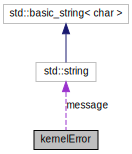
\includegraphics[width=204pt]{dc/df6/structkernelError__coll__graph}
\end{center}
\end{figure}
\subsection*{\-Public \-Attributes}
\begin{DoxyCompactItemize}
\item 
\hypertarget{structkernelError_a047e3e93719a3267825e891fe9285981}{string {\bfseries message}}\label{dc/d4b/structkernelError_a047e3e93719a3267825e891fe9285981}

\end{DoxyCompactItemize}


\subsection{\-Detailed \-Description}
\-When the kernel crashes, important information is placed in here and then handled by the main function in init.\-cpp. 

\-The documentation for this struct was generated from the following file\-:\begin{DoxyCompactItemize}
\item 
include/\hyperlink{kernel_8h}{kernel.\-h}\end{DoxyCompactItemize}

\hypertarget{structProcessInfo}{\section{\-Process\-Info \-Struct \-Reference}
\label{dd/dc8/structProcessInfo}\index{\-Process\-Info@{\-Process\-Info}}
}


\-Structure for containing process state and data.  




{\ttfamily \#include $<$process.\-h$>$}

\subsection*{\-Public \-Attributes}
\begin{DoxyCompactItemize}
\item 
\hypertarget{structProcessInfo_a102b9e7e7d958b508cec182bbcaf7d85}{unsigned int {\bfseries parent}}\label{dd/dc8/structProcessInfo_a102b9e7e7d958b508cec182bbcaf7d85}

\item 
\hypertarget{structProcessInfo_ab522cec1e6f7f3b6a7780e6b4611c1f4}{unsigned int {\bfseries pid}}\label{dd/dc8/structProcessInfo_ab522cec1e6f7f3b6a7780e6b4611c1f4}

\item 
\hypertarget{structProcessInfo_ac1e6244dd31274040bdf7ad7ee40db4a}{unsigned int {\bfseries start\-C\-P\-U}}\label{dd/dc8/structProcessInfo_ac1e6244dd31274040bdf7ad7ee40db4a}

\item 
\hypertarget{structProcessInfo_a8a6eda10132e07b1596c09822724b0c7}{unsigned int {\bfseries total\-C\-P\-U}}\label{dd/dc8/structProcessInfo_a8a6eda10132e07b1596c09822724b0c7}

\item 
\hypertarget{structProcessInfo_a748790bb8c3ef5d2dff552f35b81298e}{\hyperlink{process_8h_a2c72cb00af5be695c1f898162350821f}{e\-Proc\-State} {\bfseries state}}\label{dd/dc8/structProcessInfo_a748790bb8c3ef5d2dff552f35b81298e}

\item 
\hypertarget{structProcessInfo_af818acf9075de7c0100858908bcc2867}{uint16\-\_\-t {\bfseries \-P\-S\-W}}\label{dd/dc8/structProcessInfo_af818acf9075de7c0100858908bcc2867}

\item 
\hypertarget{structProcessInfo_a2f9f55dc3548d0bed66e06db8f47d958}{int {\bfseries priority}}\label{dd/dc8/structProcessInfo_a2f9f55dc3548d0bed66e06db8f47d958}

\item 
\hypertarget{structProcessInfo_a9b2d3f321f21ec1ee97c8dd5e63ac6c8}{unsigned int {\bfseries \-P\-C}}\label{dd/dc8/structProcessInfo_a9b2d3f321f21ec1ee97c8dd5e63ac6c8}

\item 
\hypertarget{structProcessInfo_ab288b59e794cb506663e22c680e05c2d}{int {\bfseries \-V\-C}}\label{dd/dc8/structProcessInfo_ab288b59e794cb506663e22c680e05c2d}

\item 
\hypertarget{structProcessInfo_ae99b529cb79a446c0ff0d1a851b67fc5}{char $\ast$ {\bfseries process\-Text}}\label{dd/dc8/structProcessInfo_ae99b529cb79a446c0ff0d1a851b67fc5}

\item 
void $\ast$ \hyperlink{structProcessInfo_aea1c50ae92f6421ae5c94ac674c1877a}{schedule\-Data}
\begin{DoxyCompactList}\small\item\em \-Scheduler specific data. \end{DoxyCompactList}\item 
\hypertarget{structProcessInfo_aa65ed051998c0493b68feeea5ae4955f}{unsigned long {\bfseries memory}}\label{dd/dc8/structProcessInfo_aa65ed051998c0493b68feeea5ae4955f}

\end{DoxyCompactItemize}


\subsection{\-Detailed \-Description}
\-This struture is created in the kernel when a process is initialized. \-It contains all process data needed for execution and for the kernel/scheduler to make desciions on it. 

\subsection{\-Member \-Data \-Documentation}
\hypertarget{structProcessInfo_aea1c50ae92f6421ae5c94ac674c1877a}{\index{\-Process\-Info@{\-Process\-Info}!schedule\-Data@{schedule\-Data}}
\index{schedule\-Data@{schedule\-Data}!ProcessInfo@{\-Process\-Info}}
\subsubsection[{schedule\-Data}]{\setlength{\rightskip}{0pt plus 5cm}void$\ast$ {\bf \-Process\-Info\-::schedule\-Data}}}\label{dd/dc8/structProcessInfo_aea1c50ae92f6421ae5c94ac674c1877a}
\-Check specific scheduler docs for the contents of this pointer. \-Since the process struct remains static, this gives the ability for schedulers to store their own state without the kernel having to know ahead of time. 

\-The documentation for this struct was generated from the following file\-:\begin{DoxyCompactItemize}
\item 
include/\hyperlink{process_8h}{process.\-h}\end{DoxyCompactItemize}

\chapter{\-File \-Documentation}
\hypertarget{cpu_8h}{\section{include/cpu.h \-File \-Reference}
\label{dc/da7/cpu_8h}\index{include/cpu.\-h@{include/cpu.\-h}}
}
{\ttfamily \#include \char`\"{}mmu.\-h\char`\"{}}\*
{\ttfamily \#include \char`\"{}data\-\_\-structs.\-h\char`\"{}}\*
{\ttfamily \#include \char`\"{}ini\-Reader.\-h\char`\"{}}\*
{\ttfamily \#include \char`\"{}utility/logger.\-h\char`\"{}}\*
{\ttfamily \#include \char`\"{}vmm\-\_\-core.\-h\char`\"{}}\*
\-Include dependency graph for cpu.\-h\-:\nopagebreak
\begin{figure}[H]
\begin{center}
\leavevmode
\includegraphics[width=350pt]{d4/d37/cpu_8h__incl}
\end{center}
\end{figure}
\-This graph shows which files directly or indirectly include this file\-:\nopagebreak
\begin{figure}[H]
\begin{center}
\leavevmode
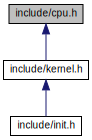
\includegraphics[width=350pt]{d8/de6/cpu_8h__dep__incl}
\end{center}
\end{figure}
\subsection*{\-Classes}
\begin{DoxyCompactItemize}
\item 
class \hyperlink{classcCPU}{c\-C\-P\-U}
\begin{DoxyCompactList}\small\item\em \-Very \-Simple \-C\-P\-U. \end{DoxyCompactList}\end{DoxyCompactItemize}
\subsection*{\-Enumerations}
\begin{DoxyCompactItemize}
\item 
enum \hyperlink{cpu_8h_a79dd30df748ae6e82b07d59888cbf05a}{e\-C\-P\-U\-State} \{ \*
\hyperlink{cpu_8h_a79dd30df748ae6e82b07d59888cbf05aaa252df7bb52b9092b5a403bd773c4ab7}{\-C\-P\-U\-\_\-\-O\-K} =  0x1, 
\hyperlink{cpu_8h_a79dd30df748ae6e82b07d59888cbf05aaae42c2aa12e3045e16b4170ce1985369}{\-C\-P\-U\-\_\-\-P\-F} =  \-C\-P\-U\-\_\-\-O\-K $<$$<$ 1, 
\hyperlink{cpu_8h_a79dd30df748ae6e82b07d59888cbf05aa358293772016df0374d4a3760e45c4f2}{\-C\-P\-U\-\_\-\-T\-E\-R\-M} =  \-C\-P\-U\-\_\-\-P\-F $<$$<$ 1, 
\hyperlink{cpu_8h_a79dd30df748ae6e82b07d59888cbf05aa254be8e08491090445866214398e163c}{\-C\-P\-U\-\_\-\-E\-X} =  \-C\-P\-U\-\_\-\-T\-E\-R\-M $<$$<$ 1, 
\*
\hyperlink{cpu_8h_a79dd30df748ae6e82b07d59888cbf05aa5fd7a8485d51f46b6dc88dba870c2e65}{\-C\-P\-U\-\_\-\-C\-I\-R\-C\-\_\-\-P\-F} =  \-C\-P\-U\-\_\-\-E\-X $<$$<$ 1
 \}
\begin{DoxyCompactList}\small\item\em \-Status of the execution quantum termination. \end{DoxyCompactList}\end{DoxyCompactItemize}


\subsection{\-Detailed \-Description}


\subsection{\-Enumeration \-Type \-Documentation}
\hypertarget{cpu_8h_a79dd30df748ae6e82b07d59888cbf05a}{\index{cpu.\-h@{cpu.\-h}!e\-C\-P\-U\-State@{e\-C\-P\-U\-State}}
\index{e\-C\-P\-U\-State@{e\-C\-P\-U\-State}!cpu.h@{cpu.\-h}}
\subsubsection[{e\-C\-P\-U\-State}]{\setlength{\rightskip}{0pt plus 5cm}enum {\bf e\-C\-P\-U\-State}}}\label{dc/da7/cpu_8h_a79dd30df748ae6e82b07d59888cbf05a}
\begin{Desc}
\item[\-Enumerator\-: ]\par
\begin{description}
\index{\-C\-P\-U\-\_\-\-O\-K@{\-C\-P\-U\-\_\-\-O\-K}!cpu.\-h@{cpu.\-h}}\index{cpu.\-h@{cpu.\-h}!\-C\-P\-U\-\_\-\-O\-K@{\-C\-P\-U\-\_\-\-O\-K}}\item[{\em 
\hypertarget{cpu_8h_a79dd30df748ae6e82b07d59888cbf05aaa252df7bb52b9092b5a403bd773c4ab7}{\-C\-P\-U\-\_\-\-O\-K}\label{dc/da7/cpu_8h_a79dd30df748ae6e82b07d59888cbf05aaa252df7bb52b9092b5a403bd773c4ab7}
}]\-C\-P\-U finished executing instruction ok. \index{\-C\-P\-U\-\_\-\-P\-F@{\-C\-P\-U\-\_\-\-P\-F}!cpu.\-h@{cpu.\-h}}\index{cpu.\-h@{cpu.\-h}!\-C\-P\-U\-\_\-\-P\-F@{\-C\-P\-U\-\_\-\-P\-F}}\item[{\em 
\hypertarget{cpu_8h_a79dd30df748ae6e82b07d59888cbf05aaae42c2aa12e3045e16b4170ce1985369}{\-C\-P\-U\-\_\-\-P\-F}\label{dc/da7/cpu_8h_a79dd30df748ae6e82b07d59888cbf05aaae42c2aa12e3045e16b4170ce1985369}
}]\-C\-P\-U/\-M\-M\-U incured a page fault. \index{\-C\-P\-U\-\_\-\-T\-E\-R\-M@{\-C\-P\-U\-\_\-\-T\-E\-R\-M}!cpu.\-h@{cpu.\-h}}\index{cpu.\-h@{cpu.\-h}!\-C\-P\-U\-\_\-\-T\-E\-R\-M@{\-C\-P\-U\-\_\-\-T\-E\-R\-M}}\item[{\em 
\hypertarget{cpu_8h_a79dd30df748ae6e82b07d59888cbf05aa358293772016df0374d4a3760e45c4f2}{\-C\-P\-U\-\_\-\-T\-E\-R\-M}\label{dc/da7/cpu_8h_a79dd30df748ae6e82b07d59888cbf05aa358293772016df0374d4a3760e45c4f2}
}]\-Process execution termination. \index{\-C\-P\-U\-\_\-\-E\-X@{\-C\-P\-U\-\_\-\-E\-X}!cpu.\-h@{cpu.\-h}}\index{cpu.\-h@{cpu.\-h}!\-C\-P\-U\-\_\-\-E\-X@{\-C\-P\-U\-\_\-\-E\-X}}\item[{\em 
\hypertarget{cpu_8h_a79dd30df748ae6e82b07d59888cbf05aa254be8e08491090445866214398e163c}{\-C\-P\-U\-\_\-\-E\-X}\label{dc/da7/cpu_8h_a79dd30df748ae6e82b07d59888cbf05aa254be8e08491090445866214398e163c}
}]\-Process exception. \index{\-C\-P\-U\-\_\-\-C\-I\-R\-C\-\_\-\-P\-F@{\-C\-P\-U\-\_\-\-C\-I\-R\-C\-\_\-\-P\-F}!cpu.\-h@{cpu.\-h}}\index{cpu.\-h@{cpu.\-h}!\-C\-P\-U\-\_\-\-C\-I\-R\-C\-\_\-\-P\-F@{\-C\-P\-U\-\_\-\-C\-I\-R\-C\-\_\-\-P\-F}}\item[{\em 
\hypertarget{cpu_8h_a79dd30df748ae6e82b07d59888cbf05aa5fd7a8485d51f46b6dc88dba870c2e65}{\-C\-P\-U\-\_\-\-C\-I\-R\-C\-\_\-\-P\-F}\label{dc/da7/cpu_8h_a79dd30df748ae6e82b07d59888cbf05aa5fd7a8485d51f46b6dc88dba870c2e65}
}]\-Potential circular page fault detected by cpu. \end{description}
\end{Desc}


\hypertarget{block__device_8h}{\section{include/devices/block\-\_\-device.h \-File \-Reference}
\label{db/d9a/block__device_8h}\index{include/devices/block\-\_\-device.\-h@{include/devices/block\-\_\-device.\-h}}
}
{\ttfamily \#include \char`\"{}devices/abstract\-\_\-device.\-h\char`\"{}}\*
\-Include dependency graph for block\-\_\-device.\-h\-:\nopagebreak
\begin{figure}[H]
\begin{center}
\leavevmode
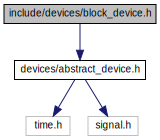
\includegraphics[width=232pt]{d7/d64/block__device_8h__incl}
\end{center}
\end{figure}
\-This graph shows which files directly or indirectly include this file\-:\nopagebreak
\begin{figure}[H]
\begin{center}
\leavevmode
\includegraphics[width=232pt]{df/dd1/block__device_8h__dep__incl}
\end{center}
\end{figure}
\subsection*{\-Classes}
\begin{DoxyCompactItemize}
\item 
class \hyperlink{classBlockDevice}{\-Block\-Device}
\end{DoxyCompactItemize}
\subsection*{\-Defines}
\begin{DoxyCompactItemize}
\item 
\hypertarget{block__device_8h_a40b115b8cd111feee88bd339876e7941}{\#define \hyperlink{block__device_8h_a40b115b8cd111feee88bd339876e7941}{\-B\-L\-O\-C\-K\-S\-I\-G}~\-S\-I\-G\-R\-T\-M\-I\-N + 1}\label{db/d9a/block__device_8h_a40b115b8cd111feee88bd339876e7941}

\begin{DoxyCompactList}\small\item\em \-Signal generated by \hyperlink{classBlockDevice}{\-Block\-Device}. \end{DoxyCompactList}\end{DoxyCompactItemize}


\subsection{\-Detailed \-Description}

\hypertarget{char__device_8h}{\section{include/devices/char\-\_\-device.h \-File \-Reference}
\label{d7/d59/char__device_8h}\index{include/devices/char\-\_\-device.\-h@{include/devices/char\-\_\-device.\-h}}
}
{\ttfamily \#include $<$cstdio$>$}\*
{\ttfamily \#include \char`\"{}devices/queued\-\_\-device.\-h\char`\"{}}\*
\-Include dependency graph for char\-\_\-device.\-h\-:\nopagebreak
\begin{figure}[H]
\begin{center}
\leavevmode
\includegraphics[width=350pt]{da/d18/char__device_8h__incl}
\end{center}
\end{figure}
\-This graph shows which files directly or indirectly include this file\-:\nopagebreak
\begin{figure}[H]
\begin{center}
\leavevmode
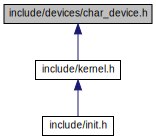
\includegraphics[width=228pt]{db/ded/char__device_8h__dep__incl}
\end{center}
\end{figure}
\subsection*{\-Classes}
\begin{DoxyCompactItemize}
\item 
class \hyperlink{classcCharDevice}{c\-Char\-Device}
\begin{DoxyCompactList}\small\item\em \-Queued char device. \end{DoxyCompactList}\end{DoxyCompactItemize}
\subsection*{\-Defines}
\begin{DoxyCompactItemize}
\item 
\hypertarget{char__device_8h_a2e6614e57b804a24ff80f29b9e840788}{\#define \hyperlink{char__device_8h_a2e6614e57b804a24ff80f29b9e840788}{\-C\-H\-A\-R\-S\-I\-G}~\-S\-I\-G\-R\-T\-M\-I\-N + 2}\label{d7/d59/char__device_8h_a2e6614e57b804a24ff80f29b9e840788}

\begin{DoxyCompactList}\small\item\em \-Signal generated by \-Char\-Device. \end{DoxyCompactList}\end{DoxyCompactItemize}


\subsection{\-Detailed \-Description}

\hypertarget{clock__device_8h}{\section{include/devices/clock\-\_\-device.h \-File \-Reference}
\label{df/d8f/clock__device_8h}\index{include/devices/clock\-\_\-device.\-h@{include/devices/clock\-\_\-device.\-h}}
}
{\ttfamily \#include $<$errno.\-h$>$}\*
{\ttfamily \#include $<$cstring$>$}\*
{\ttfamily \#include $<$string$>$}\*
{\ttfamily \#include \char`\"{}devices/abstract\-\_\-device.\-h\char`\"{}}\*
\-Include dependency graph for clock\-\_\-device.\-h\-:\nopagebreak
\begin{figure}[H]
\begin{center}
\leavevmode
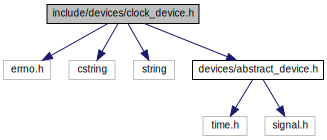
\includegraphics[width=350pt]{db/d16/clock__device_8h__incl}
\end{center}
\end{figure}
\-This graph shows which files directly or indirectly include this file\-:\nopagebreak
\begin{figure}[H]
\begin{center}
\leavevmode
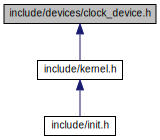
\includegraphics[width=232pt]{d8/d7f/clock__device_8h__dep__incl}
\end{center}
\end{figure}
\subsection*{\-Classes}
\begin{DoxyCompactItemize}
\item 
class \hyperlink{classClockDevice}{\-Clock\-Device}
\end{DoxyCompactItemize}
\subsection*{\-Defines}
\begin{DoxyCompactItemize}
\item 
\hypertarget{clock__device_8h_a2694a39dfd1fa087ca6f9f391c91dae7}{\#define {\bfseries \-C\-L\-O\-C\-K\-I\-D}~\-C\-L\-O\-C\-K\-\_\-\-R\-E\-A\-L\-T\-I\-M\-E}\label{df/d8f/clock__device_8h_a2694a39dfd1fa087ca6f9f391c91dae7}

\item 
\hypertarget{clock__device_8h_af6318deadd0687fb8ffb5437eaa1870d}{\#define \hyperlink{clock__device_8h_af6318deadd0687fb8ffb5437eaa1870d}{\-C\-L\-O\-C\-K\-S\-I\-G}~\-S\-I\-G\-R\-T\-M\-I\-N}\label{df/d8f/clock__device_8h_af6318deadd0687fb8ffb5437eaa1870d}

\begin{DoxyCompactList}\small\item\em \-Signal generated by \hyperlink{classClockDevice}{\-Clock\-Device}. \end{DoxyCompactList}\end{DoxyCompactItemize}


\subsection{\-Detailed \-Description}

\hypertarget{kernel_8h}{\section{include/kernel.h \-File \-Reference}
\label{d0/daa/kernel_8h}\index{include/kernel.\-h@{include/kernel.\-h}}
}
{\ttfamily \#include $<$vector$>$}\*
{\ttfamily \#include $<$fcntl.\-h$>$}\*
{\ttfamily \#include $<$sys/types.\-h$>$}\*
{\ttfamily \#include $<$sys/stat.\-h$>$}\*
{\ttfamily \#include \char`\"{}cpu.\-h\char`\"{}}\*
{\ttfamily \#include \char`\"{}devices/char\-\_\-device.\-h\char`\"{}}\*
{\ttfamily \#include \char`\"{}devices/block\-\_\-device.\-h\char`\"{}}\*
{\ttfamily \#include \char`\"{}devices/clock\-\_\-device.\-h\char`\"{}}\*
{\ttfamily \#include \char`\"{}utility/id.\-h\char`\"{}}\*
{\ttfamily \#include \char`\"{}scheduler/fcfs.\-h\char`\"{}}\*
\-Include dependency graph for kernel.\-h\-:
\nopagebreak
\begin{figure}[H]
\begin{center}
\leavevmode
\includegraphics[width=350pt]{d4/d0f/kernel_8h__incl}
\end{center}
\end{figure}
\-This graph shows which files directly or indirectly include this file\-:\nopagebreak
\begin{figure}[H]
\begin{center}
\leavevmode
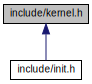
\includegraphics[width=164pt]{de/df8/kernel_8h__dep__incl}
\end{center}
\end{figure}
\subsection*{\-Classes}
\begin{DoxyCompactItemize}
\item 
class \hyperlink{classcKernel}{c\-Kernel}
\end{DoxyCompactItemize}
\subsection*{\-Defines}
\begin{DoxyCompactItemize}
\item 
\hypertarget{kernel_8h_ac91bd56eef3f2b82894a058b7f136a21}{\#define {\bfseries \-D\-E\-F\-A\-U\-L\-T\-\_\-\-T\-I\-M\-E\-R}~1000}\label{d0/daa/kernel_8h_ac91bd56eef3f2b82894a058b7f136a21}

\item 
\hypertarget{kernel_8h_a0756f011ef667460d583017366823244}{\#define {\bfseries \-D\-E\-F\-A\-U\-L\-T\-\_\-\-P\-R\-I\-O\-R\-I\-T\-Y}~0}\label{d0/daa/kernel_8h_a0756f011ef667460d583017366823244}

\end{DoxyCompactItemize}
\subsection*{\-Typedefs}
\begin{DoxyCompactItemize}
\item 
\hypertarget{kernel_8h_a87e7ee09eb9354187e1877a668567104}{typedef \hyperlink{classcFCFS}{c\-F\-C\-F\-S} {\bfseries scheduler\-Type}}\label{d0/daa/kernel_8h_a87e7ee09eb9354187e1877a668567104}

\end{DoxyCompactItemize}
\subsection*{\-Functions}
\begin{DoxyCompactItemize}
\item 
\hypertarget{kernel_8h_a0847dda36bbd7bf064de17946b4239a7}{{\bfseries \-\_\-\-\_\-attribute\-\_\-\-\_\-} ((error(\char`\"{}process.\-h not included by scheduler\char`\"{})))}\label{d0/daa/kernel_8h_a0847dda36bbd7bf064de17946b4239a7}

\end{DoxyCompactItemize}


\subsection{\-Detailed \-Description}

\hypertarget{process_8h}{\section{include/process.h \-File \-Reference}
\label{da/d42/process_8h}\index{include/process.\-h@{include/process.\-h}}
}
{\ttfamily \#include $<$inttypes.\-h$>$}\*
\-Include dependency graph for process.\-h\-:\nopagebreak
\begin{figure}[H]
\begin{center}
\leavevmode
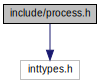
\includegraphics[width=172pt]{d5/dab/process_8h__incl}
\end{center}
\end{figure}
\-This graph shows which files directly or indirectly include this file\-:\nopagebreak
\begin{figure}[H]
\begin{center}
\leavevmode
\includegraphics[width=350pt]{d1/d54/process_8h__dep__incl}
\end{center}
\end{figure}
\subsection*{\-Classes}
\begin{DoxyCompactItemize}
\item 
struct \hyperlink{structProcessInfo}{\-Process\-Info}
\begin{DoxyCompactList}\small\item\em \-Structure for containing process state and data. \end{DoxyCompactList}\end{DoxyCompactItemize}
\subsection*{\-Typedefs}
\begin{DoxyCompactItemize}
\item 
\hypertarget{process_8h_a1c804f1220f3edf8f809fa0ccfb7643f}{typedef unsigned int {\bfseries pid\-Type}}\label{da/d42/process_8h_a1c804f1220f3edf8f809fa0ccfb7643f}

\end{DoxyCompactItemize}
\subsection*{\-Enumerations}
\begin{DoxyCompactItemize}
\item 
enum \hyperlink{process_8h_a2c72cb00af5be695c1f898162350821f}{e\-Proc\-State} \{ \hyperlink{process_8h_a2c72cb00af5be695c1f898162350821fa3d4001ca586c857718be397374082d76}{ready}, 
\hyperlink{process_8h_a2c72cb00af5be695c1f898162350821faf9ccc71a0c4e71cc139d2c885154b243}{running}, 
\hyperlink{process_8h_a2c72cb00af5be695c1f898162350821fa035732e2026cb263f1bd9eee6ca6ae01}{blocked}, 
\hyperlink{process_8h_a2c72cb00af5be695c1f898162350821fa21b6f86c6d8b11d4a9c163130f55c5dd}{terminated}
 \}
\begin{DoxyCompactList}\small\item\em \-Enumeration for process states. \end{DoxyCompactList}\end{DoxyCompactItemize}


\subsection{\-Detailed \-Description}


\subsection{\-Enumeration \-Type \-Documentation}
\hypertarget{process_8h_a2c72cb00af5be695c1f898162350821f}{\index{process.\-h@{process.\-h}!e\-Proc\-State@{e\-Proc\-State}}
\index{e\-Proc\-State@{e\-Proc\-State}!process.h@{process.\-h}}
\subsubsection[{e\-Proc\-State}]{\setlength{\rightskip}{0pt plus 5cm}enum {\bf e\-Proc\-State}}}\label{da/d42/process_8h_a2c72cb00af5be695c1f898162350821f}
\-Each values defines a current state and possible transitions. \begin{Desc}
\item[\-Enumerator\-: ]\par
\begin{description}
\index{ready@{ready}!process.\-h@{process.\-h}}\index{process.\-h@{process.\-h}!ready@{ready}}\item[{\em 
\hypertarget{process_8h_a2c72cb00af5be695c1f898162350821fa3d4001ca586c857718be397374082d76}{ready}\label{da/d42/process_8h_a2c72cb00af5be695c1f898162350821fa3d4001ca586c857718be397374082d76}
}]\-Process is ready to be run. \-Invariant \-State\-:\par
 \begin{DoxyItemize}
\item \-Kernel has initialized it at some point \item \-Process should be preparred to run\end{DoxyItemize}
\-Potential \-Transitions\-: \begin{DoxyItemize}
\item \hyperlink{process_8h_a2c72cb00af5be695c1f898162350821faf9ccc71a0c4e71cc139d2c885154b243}{running} -\/ \-Scheduler picks it to run next \end{DoxyItemize}
\index{running@{running}!process.\-h@{process.\-h}}\index{process.\-h@{process.\-h}!running@{running}}\item[{\em 
\hypertarget{process_8h_a2c72cb00af5be695c1f898162350821faf9ccc71a0c4e71cc139d2c885154b243}{running}\label{da/d42/process_8h_a2c72cb00af5be695c1f898162350821faf9ccc71a0c4e71cc139d2c885154b243}
}]\-Process is currently running. \-A running process should implicilty be considered ready. \-The kernel may not notify the scheduler to transition the process to ready before asking for a a scheduling decision. \-It is acceptable for the scheduler to make a process ready without the kernel's consent when it is being asked for a scheduling decision, assuming it was previously running.

\-Invariant \-State\-: \begin{DoxyItemize}
\item \-Process is on the cpu\end{DoxyItemize}
\-Potential \-Transitions\-: \begin{DoxyItemize}
\item \hyperlink{process_8h_a2c72cb00af5be695c1f898162350821fa3d4001ca586c857718be397374082d76}{ready} -\/ \-Scheduler picks someone else to run \item \hyperlink{process_8h_a2c72cb00af5be695c1f898162350821fa035732e2026cb263f1bd9eee6ca6ae01}{blocked} -\/ \-Makes blocking system call \item \hyperlink{process_8h_a2c72cb00af5be695c1f898162350821fa21b6f86c6d8b11d4a9c163130f55c5dd}{terminated} -\/ \-Causes exception in cpu or finished normally \end{DoxyItemize}
\index{blocked@{blocked}!process.\-h@{process.\-h}}\index{process.\-h@{process.\-h}!blocked@{blocked}}\item[{\em 
\hypertarget{process_8h_a2c72cb00af5be695c1f898162350821fa035732e2026cb263f1bd9eee6ca6ae01}{blocked}\label{da/d42/process_8h_a2c72cb00af5be695c1f898162350821fa035732e2026cb263f1bd9eee6ca6ae01}
}]\-Process is blocked and cannot run. \-Invariant \-State\-: \begin{DoxyItemize}
\item \-Process is blocked (for now it can only block on \-I/\-O)\end{DoxyItemize}
\-Potential \-Transitions\-: \begin{DoxyItemize}
\item \hyperlink{process_8h_a2c72cb00af5be695c1f898162350821fa3d4001ca586c857718be397374082d76}{ready} -\/ \-Kernel notifies scheduler that \-I/\-O has finished \end{DoxyItemize}
\index{terminated@{terminated}!process.\-h@{process.\-h}}\index{process.\-h@{process.\-h}!terminated@{terminated}}\item[{\em 
\hypertarget{process_8h_a2c72cb00af5be695c1f898162350821fa21b6f86c6d8b11d4a9c163130f55c5dd}{terminated}\label{da/d42/process_8h_a2c72cb00af5be695c1f898162350821fa21b6f86c6d8b11d4a9c163130f55c5dd}
}]\-Process has been terminated. \-It will be cleaned up soon.

\-Invariant \-State\-: \begin{DoxyItemize}
\item \-Process either caused cpu exception or finished \item \-Process can no longer run\end{DoxyItemize}
\-Potential \-Transitions\-: \begin{DoxyItemize}
\item \-None \end{DoxyItemize}
\end{description}
\end{Desc}


\printindex
\end{document}
